\section{2024年普通高等学校招生全国统一考试(新高考2卷)}
\parttitle{单选题}
\begin{example}{1}[2024][全国2卷][高三][高考][第1题]
已知$z=-1-i$，则$|z|=\blankbox$
\begin{choices}
\choice{$0$}
\choice{$1$}
\choice{$\sqrt{2}$}
\choice{$2$}
\end{choices}
\end{example}

\begin{example}{1}[2024][全国2卷][高三][高考][第2题]
已知命题$p$：$\forall x\in R$，$|x+1|>1$；命题$q$：$\exists x>0$，$x^3=x$，则$\blankbox$
\begin{choices}
\choice{$p$和$q$都是真命题}
\choice{$\neg p$和$q$都是真命题}
\choice{$p$和$\neg q$都是真命题}
\choice{$\neg p$和$\neg q$都是真命题}
\end{choices}
\end{example}

\begin{example}{1}[2024][全国2卷][高三][高考][第3题]
已知向量$\vec{a}$，$\vec{b}$满足$|\vec{a}|=1$，$|\vec{a}+2\vec{b}|=2$，且$(\vec{b}-2\vec{a})\perp\vec{b}$，则$|\vec{b}|=\blankbox$
\begin{choices}
\choice{$\dfrac{1}{2}$}
\choice{$\dfrac{\sqrt{2}}{2}$}
\choice{$\dfrac{\sqrt{3}}{2}$}
\choice{$1$}
\end{choices}
\end{example}

\begin{example}{1}[2024][全国2卷][高三][高考][第4题]
某农业研究部门在面积相等的100块稻田上种植一种新型水稻，得到各块稻田的亩产量（单位：kg）并部分整理如下表：
\begin{center}
\begin{tabular}{|c|c|c|c|c|c|}
\hline
亩产量 & $[900,950)$ & $[950,1000)$ & $[1000,1050)$ & $[1100,1150)$ & $[1150,1200)$ \\
\hline
频数 & 6 & 12 & 18 & 24 & 10 \\
\hline
\end{tabular}
\end{center}
据表中数据，结论中正确的是$\blankbox$
\begin{choices}
\choice{100块稻田亩产量的中位数小于1050kg}
\choice{100块稻田中亩产量低于1100kg的稻田所占比例超过80\%}
\choice{100块稻田亩产量的极差介于200kg至300kg之间}
\choice{100块稻田亩产量的平均值介于900kg至1000kg之间}
\end{choices}
\end{example}

\begin{example}{1}[2024][全国2卷][高三][高考][第5题]
已知曲线$C$：$x^2+y^2=16(y>0)$，从$C$上任意一点$P$向$x$轴作垂线段$PP'$，$P'$为垂足，则线段$PP'$的中点$M$的轨迹方程为$\blankbox$
\begin{choices}
\choice{$\dfrac{x^2}{16}+\dfrac{y^2}{4}=1(y>0)$}
\choice{$\dfrac{x^2}{16}+\dfrac{y^2}{8}=1(y>0)$}
\choice{$\dfrac{y^2}{16}+\dfrac{x^2}{4}=1(y>0)$}
\choice{$\dfrac{y^2}{16}+\dfrac{x^2}{8}=1(y>0)$}
\end{choices}
\end{example}

\begin{example}{1}[2024][全国2卷][高三][高考][第6题]
设函数$f(x)=a(x+1)^2-1$，$g(x)=\cos x+2ax$，当$x\in(-1,1)$时，曲线$y=f(x)$与$y=g(x)$恰有一个交点，则$a=\blankbox$
\begin{choices}
\choice{$-1$}
\choice{$\dfrac{1}{2}$}
\choice{$1$}
\choice{$2$}
\end{choices}
\end{example}

\begin{example}{1}[2024][全国2卷][高三][高考][第7题]
已知正三棱台$ABC-A_1B_1C_1$的体积为$\dfrac{52}{3}$，$AB=6$，$A_1B_1=2$，则$A_1A$与平面$ABC$所成角的正切值为$\blankbox$
\begin{choices}
\choice{$\dfrac{1}{2}$}
\choice{$1$}
\choice{$2$}
\choice{$3$}
\end{choices}
\end{example}

\begin{example}{1}[2024][全国2卷][高三][高考][第8题]
设函数$f(x)=(x+a)\ln(x+b)$，若$f(x)\ge 0$，则$a^2+b^2$的最小值为$\blankbox$
\begin{choices}
\choice{$\dfrac{1}{8}$}
\choice{$\dfrac{1}{4}$}
\choice{$\dfrac{1}{2}$}
\choice{$1$}
\end{choices}
\end{example}
\parttitle{多选题}
\begin{example}{2}[2024][全国2卷][高三][高考][第9题][多选]
对于函数$f(x)=\sin 2x$和$g(x)=\sin\left(2x-\dfrac{\pi}{4}\right)$，下列正确的有$\blankbox$
\begin{choices}
\choice{$f(x)$与$g(x)$有相同零点}
\choice{$f(x)$与$g(x)$有相同最大值}
\choice{$f(x)$与$g(x)$有相同的最小正周期}
\choice{$f(x)$与$g(x)$的图像有相同的对称轴}
\end{choices}
\end{example}

\begin{example}{2}[2024][全国2卷][高三][高考][第10题][多选]
抛物线$C$：$y^2=4x$的准线为$l$，$P$为$C$上的动点，过$P$作$\odot A$：$x^2+(y-4)^2=1$的一条切线，$Q$为切点，过$P$作$l$的垂线，垂足为$B$，则$\blankbox$
\begin{choices}
\choice{$l$与$\odot A$相切}
\choice{当$P,A,B$三点共线时，$|PQ|=\sqrt{15}$}
\choice{当$|PB|=2$时，$PA\perp AB$}
\choice{满足$|PA|=|PB|$的点$P$有且仅有2个}
\end{choices}
\end{example}

\begin{example}{2}[2024][全国2卷][高三][高考][第11题][多选]
设函数$f(x)=2x^3-3ax^2+1$，则$\blankbox$
\begin{choices}
\choice{当$a>1$时，$f(x)$有三个零点}
\choice{当$a<0$时，$x=0$是$f(x)$的极大值点}
\choice{存在$a,b$，使得$x=b$为曲线$y=f(x)$的对称轴}
\choice{存在$a$，使得点$(1,f(1))$为曲线$y=f(x)$的对称中心}
\end{choices}
\end{example}
\parttitle{填空题}
\begin{example}{3}[2024][全国2卷][高三][高考][第12题]
记$S_n$为等差数列$\{a_n\}$的前$n$项和，若$a_3+a_4=7$，$3a_2+a_5=5$，则$S_{10}=\blankline$
\end{example}

\begin{example}{3}[2024][全国2卷][高三][高考][第13题]
已知$\alpha$为第一象限角，$\beta$为第三象限角，$\tan\alpha+\tan\beta=4$，$\tan\alpha\tan\beta=\sqrt{2}+1$，则$\sin(\alpha+\beta)=\blankline$
\end{example}

\begin{example}{3}[2024][全国2卷][高三][高考][第14题]
在如图的4×4方格表中选4个方格，要求每行和每列均恰有一个方格被选中，则共有$\blankline$种选法；在所有符合上述要求的选法中，选中方格中的4个数之和的最大值是$\blankline$
\begin{center}
\begin{tabular}{|c|c|c|c|}
\hline
11 & 21 & 31 & 40 \\
\hline
12 & 22 & 33 & 42 \\
\hline
13 & 22 & 33 & 43 \\
\hline
15 & 24 & 34 & 44 \\
\hline
\end{tabular}
\end{center}
\end{example}
\parttitle{简答题}
\begin{example}{4}[2024][全国2卷][高三][高考][第15题]
记$\triangle ABC$的内角$A,B,C$的对边分别为$a,b,c$，已知$\sin A+\sqrt{3}\cos A=2$。
\begin{enumerate}
\item 求$A$；
\item 若$a=2$，$\sqrt{2}b\sin C=c\sin 2B$，求$\triangle ABC$的周长。
\end{enumerate}
\end{example}

\begin{example}{4}[2024][全国2卷][高三][高考][第16题]
已知函数$f(x)=e^x-ax-a^3$。
\begin{enumerate}
\item 当$a=1$时，求曲线$y=f(x)$在点$(1,f(1))$处的切线方程；
\item 若$f(x)$有极小值，且极小值小于0，求$a$的取值范围。
\end{enumerate}
\end{example}

\begin{example}{4}[2024][全国2卷][高三][高考][第17题]
如图，平面四边形$ABCD$中，$AB=8$，$CD=3$，$AD=5\sqrt{3}$，$\angle ADC=90^\circ$，$\angle BAD=30^\circ$，点$E,F$满足$\overrightarrow{AE}=\dfrac{2}{5}\overrightarrow{AD}$，$\overrightarrow{AF}=\dfrac{1}{2}\overrightarrow{AB}$。将$\triangle AEF$沿$EF$对折至$\triangle PEF$，使得$PC=4\sqrt{3}$。
\begin{enumerate}
\item 证明：$EF\perp PD$；
\item 求面$PCD$与面$PBF$所成的二面角的正弦值。
\end{enumerate}
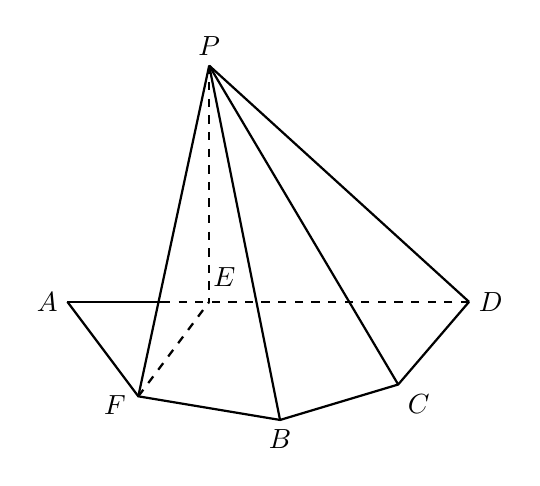
\begin{tikzpicture}[scale=1.5, >=latex]
	% 1. 定义空间各顶点的三维投影坐标（针对 C、F 进行了投影拉伸优化）
	\coordinate (E) at (0,0);
	\coordinate (D) at (2.2,0);
	\coordinate (A) at (-1.2,0);
	\coordinate (F) at (-0.6,-0.8);
	\coordinate (B) at (0.6,-1.0);
	\coordinate (C) at (1.6,-0.7);
	\coordinate (P) at (0,2.0); % P在E的正上方，天然满足 PE 垂直于底面内的 DE
		\coordinate (Q) at (-0.4,0);
	% 2. 绘制不可见线（虚线段）
	\draw[dashed,thick] (Q) -- (E);
	\draw[dashed, thick] (D) -- (E);
	\draw[dashed, thick] (F) -- (E);
	\draw[dashed, thick] (P) -- (E);
	
	% 3. 绘制可见线（实线段）
	\draw[thick] (A) -- (F) -- (B) -- (C) -- (D);
	\draw[thick] (P) -- (F);
	\draw[thick] (P) -- (B);
	\draw[thick] (P) -- (C);
	\draw[thick] (P) -- (D);
		\draw[thick] (A) -- (Q);
	% 4. 精准标注顶点字母（使用合理的 anchor 偏移，防止字母贴近线条）
	\node[above] at (P) {$P$};
	\node[above right, xshift=-2pt, yshift=2pt] at (E) {$E$};
	\node[right] at (D) {$D$};
	\node[left] at (A) {$A$};
	\node[left, xshift=-1pt, yshift=-3pt] at (F) {$F$};
	\node[below] at (B) {$B$};
	\node[below right] at (C) {$C$};
	
\end{tikzpicture}
\end{example}

\begin{example}{4}[2024][全国2卷][高三][高考][第18题]
某投篮比赛分为两个阶段，每个参赛队由两名队员组成，比赛具体规则如下：第一阶段由参赛队中一名队员投篮3次，若3次都未投中，则该队被淘汰，比赛得分为0分；若至少投中一次，则该队进入第二阶段，由该队的另一名队员投篮3次，每次投中得5分，未投中得0分。该队的比赛成绩为第二阶段的得分总和。某参赛队由甲、乙两名队员组成，设甲每次投中的概率为$p$，乙每次投中的概率为$q$，各次投中与否相互独立。
\begin{enumerate}
\item 若$p=0.4$，$q=0.5$，甲参加第一阶段比赛，求甲、乙所在队的比赛成绩不少于5分的概率。
\item 假设$0<p<q$，
\begin{enumerate}
\item 为使得甲、乙所在队的比赛成绩为15分的概率最大，应该由谁参加第一阶段比赛？
\item 为使得甲、乙所在队的比赛成绩的数学期望最大，应该由谁参加第一阶段比赛？
\end{enumerate}
\end{enumerate}
\end{example}

\begin{example}{4}[2024][全国2卷][高三][高考][第19题]
已知双曲线$C$：$x^2-y^2=m(m>0)$，点$P_1(5,4)$在$C$上，$k$为常数，$0<k<1$。按照如下方式依次构造点$P_n(n=2,3,\dots)$：过$P_{n-1}$作斜率为$k$的直线与$C$的左支交于点$Q_{n-1}$，令$P_n$为$Q_{n-1}$关于$y$轴的对称点，记$P_n$的坐标为$(x_n,y_n)$。
\begin{enumerate}
\item 若$k=\dfrac{1}{2}$，求$x_2,y_2$；
\item 证明：数列$\{x_n-y_n\}$是公比为$\dfrac{1+k}{1-k}$的等比数列；
\item 设$S_n$为$\triangle P_nP_{n+1}P_{n+2}$的面积，证明：对任意的正整数$n$，$S_n=S_{n+1}$。
\end{enumerate}
\end{example}